%-----------------------------------------------------------------------------%
\chapter{\babDua}
\label{bab:2}


\section{Masalah Pemeringkatan Teks}
    Permasalahan pemeringkatan teks adalah permasalahan untuk menentukan urutan teks yang paling relevan dengan kueri $q$ yang diberikan. Dalam bahasa yang lebih formal, diberikan kueri $q$ dan himpunan teks terbatas $\mathcal{D}= \{d_1, d_2, ..., d_n\}$, keluaran yang diinginkan dari permasalahan ini adalah barisan teks $D_k = (d_{i_1}, d_{i_2}, ..., d_{i_k})$ yang merupakan $k$ teks yang paling relevan dengan kueri $q$. Selain itu, biasanya nilai $k$ akan lebih kecil dari banyaknya teks yang ada, sehingga permasalahan pemeringkatan teks sering juga disebut sebagai \f{top-k retrieval}. Untuk mengukur performa suatu model pemeringkatan, biasanya digunakan metrik evaluasi seperti presisi, \f{recall}, \f{reciprocal rank}, dan \f{normalized discounted cumulative gain} (nDCG) yang akan dijelaskan pada \sect~\ref{sec:metrik-evaluasi}.

    \subsection{Bentuk Umum \f{Dataset}}
    \label{sec:dataset-umum}
    Sebelum menjelaskan metrik evaluasi, akan dijelaskan terlebih dahulu bentuk umum dari \f{dataset} yang digunakan untuk mengevaluasi sebuah sistem pemeringkatan teks. Bentuk umum dari \f{dataset} yang digunakan biasanya terdiri dari 3 \f{file}, yaitu \f{file} korpus, \f{file} kueri, dan \f{file judgements}. \f{File} korpus adalah kumpulan teks yang ingin di-\f{retreive} oleh sebuah sistem pemeringkatan teks. Pada \f{file} korpus terdapat 3 kolom, yaitu id teks, judul teks, dan isi dari teks tersebut. \tab~\ref{tab:contoh-file-korpus} menunjukkan potongan dari \f{file} korpus.
    \begin{table}[!ht]
        \centering
        \caption{Potongan \f{file} korpus \f{dataset} Miracl.}
        \label{tab:contoh-file-korpus}
        \begin{tabular}{|l|l|p{0.6\textwidth}|}
            \hline
            \textbf{\_id}    & \textbf{title}             & \textbf{text}                                                                                                 \\ \hline
            1342516\#1  & Colobothea biguttata & Larva kumbang ini biasanya mengebor ke dalam kayu dan dapat menyebabkan kerusakan pada batang kayu hidup atau kayu yang telah ditebang. \\ \hline
            1342517\#0  & Ichthyodes rufipes  & Ichthyodes rufipes adalah spesies kumbang tanduk panjang yang berasal dari famili Cerambycidae. Spesies ini juga merupakan bagian dari genus Ichthyodes, ordo Coleoptera, kelas Insecta, filum Arthropoda, dan kingdom Animalia. \\ \hline
        \end{tabular}
    \end{table}

    \f{File} kueri berisi kumpulan kueri yang digunakan untuk mengambil teks dari \f{file} korpus. 
    performa dari sistem pemeringkatan teks akan diukur dengan mengambil $k$ teks dari \f{file} korpus untuk setiap kueri pada \f{file} kueri. Pada \f{file} kueri terdapat 2 kolom, yaitu id kueri dan isi dari kueri tersebut. \tab~\ref{tab:query-file-example} menunjukkan potongan dari \f{file} kueri.
    \begin{table}[!ht]
        \centering
        \caption{Potongan \f{file} kueri \f{dataset} Miracl.}
        \label{tab:query-file-example}
        \begin{tabular}{|l|p{0.8\textwidth}|}
            \hline
            \textbf{\_id} & \textbf{text}                                                                 \\ \hline
            3             & Dimana James Hepburn meninggal?                                              \\ \hline
            4             & Dimana Jamie Richard Vardy lahir?                                            \\ \hline
            11            & berapakah luas pulau Flores?                                                 \\ \hline
            17            & Siapakah yang menulis Candy Candy?                                           \\ \hline
            19            & Apakah karya tulis Irma Hardisurya yang pertama?                              \\ \hline
        \end{tabular}
    \end{table}
    Selanjutnya, \f{file judgements} berisi pemetaan relevansi antara kueri pada \f{file} kueri dengan teks pada \f{file} korpus. Pada \f{file} judgements terdapat 3 kolom, yaitu id kueri, id teks, dan relevansi $r$ antara kueri dan teks tersebut. Pasangan $(\text{kueri}, \text{teks})$ yang relevan akan memiliki nilai $r > 0$ dan nilai $r$ yang makin besar menunjukkan tingkat relevansi yang makin tinggi. Selain itu, pasangan $(\text{kueri}, \text{teks})$ yang tidak relevan akan memiliki nilai $r = 0$ dan biasanya pasangan $(\text{kueri}, \text{teks})$ yang tidak relevan tidak dituliskan pada \f{file judgements}. Tak menutup kemungkinan jika sebuah \f{dataset} hanya menggunakan nilai relevansi biner ($r \in \{0, 1\}$). Terakhir, \tab~\ref{tab:judgements-file-example} menunjukkan potongan dari \f{file judgements}.
    \begin{table}[!ht]
        \centering
        \caption{Potongan \f{file} judgements \f{dataset} Miracl.}
        \label{tab:judgements-file-example}
        \begin{tabular}{|l|l|l|}
            \hline
            \textbf{query-id} & \textbf{corpus-id} & \textbf{score} \\ \hline
            3                 & 115796\#6          & 1              \\ \hline
            3                 & 77689\#48          & 1              \\ \hline
            4                 & 1852373\#0         & 1              \\ \hline
        \end{tabular}
    \end{table}
    


    \subsection{Metrik Evaluasi dalam Pemeringkatan Teks}
    \label{sec:metrik-evaluasi}
    Subbab ini menjelaskan beberapa metrik evaluasi yang sering digunakan untuk mengukur performa dari sistem pemeringkatan teks. Metrik evaluasi yang akan dijelaskan adalah \f{recall}, presisi, \f{reciprocal rank}, dan \f{normalized discounted cumulative gain} (nDCG). Metrik tersebut digunakan untuk mengukur performa dari sistem pemeringkatan teks dengan mengambil $k$ teks dari \f{file} korpus pada satu kueri. Untuk mendapatkan performa dari sistem pemeringkatan teks secara keseluruhan, biasanya metrik evaluasi tersebut akan dihitung untuk setiap kueri pada \f{file} kueri dan kemudian diambil nilai rata-ratanya.

    \subsubsection{\f{Recall} dan Presisi}

        \begin{figure}[!ht]
            \centering
            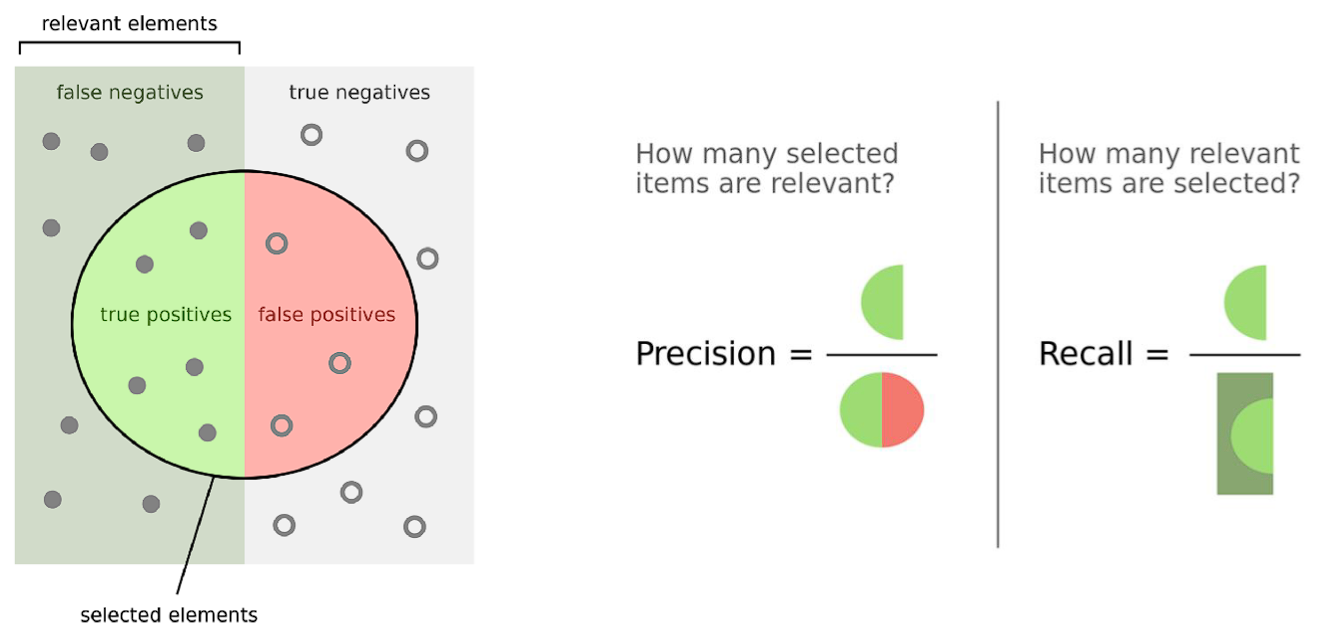
\includegraphics[width=1\textwidth]{assets/pics/recall-presisi.png}
            \captionsource{Ilustrasi \f{recall} dan presisi. Nilai \f{recall} dihitung sebagai rasio teks relevan yang diambil oleh sistem terhadap seluruh teks yang relevan dengan kueri $q$. Sedangkan nilai presisi dihitung sebagai rasio teks relevan yang diambil oleh sistem terhadap seluruh teks yang diambil oleh sistem.}{\citep{irlecture}.}
            \label{fig:recall-precision}
        \end{figure}
        Presisi dan \f{recall} adalah metrik yang paling sederhana untuk mengukur kemampuan dari suatu sistem pemeringkatan teks. \f{Recall} mengukur kemampuan sistem dalam mengembalikan semua teks yang relevan dengan kueri $q$ dari himpunan teks $\mathcal{D}$, sedangkan presisi mengukur kemampuan sistem dalam mengembalikan teks yang relevan dengan kueri $q$ dari himpunan teks $\mathcal{D}$. Untuk suatu kueri $q$, kumpulan teks $\mathcal{D} = \{d_1, d_2, ..., d_n\}$, dan barisan $k$ teks yang diambil oleh sistem, $D_k = (d_{i_1}, d_{i_2}, ..., d_{i_k})$, \f{recall} dan presisi dapat dihitung dengan \equ~\ref{eq:recall} hingga \equ~\ref{eq:presisi}.
        \begin{align}
            \label{eq:recall}
            \text{recall}(q, D_k)\text{@k} &= \frac{\sum_{d \in D_k} \text{rel}(q, d)}{\sum_{d \in \mathcal{D}} \text{rel}(q, d)} \in [0, 1], \\
            \label{eq:presisi}
            \text{precision}(q, D_k)\text{@k} &= \frac{\sum_{d \in D_k} \text{rel}(q, d)}{|D_k|} \in [0, 1], \\
            \label{eq:rel}
            \text{rel}(q, d) &= \begin{cases} 
            1 & \text{jika } r > 1 \\
            0 & \text{jika } r = 0
            \end{cases}.
        \end{align}

        Sebagai contoh, jika terdapat 10 teks yang relevan dengan kueri $q$, dan sistem mengembalikan $k=100$ teks, namun hanya terdapat 5 teks yang relevan pada $D_k$  maka \f{recall} dan presisi dari sistem tersebut adalah 0.5 ($\frac{5}{10}$) dan 0.05 ($\frac{5}{100}$) masing-masing. Baik \f{recall} maupun presisi memiliki rentang nilai dari 0 hingga 1, dengan nilai 1 menunjukkan performa sistem yang terbaik. Perhitungan \f{recall} biasanya dilakukan untuk $k$ yang cukup besar ($k = 100,1000 $), sedangkan perhitungan presisi dilakukan untuk $k$ yang kecil ($k = 1, 3, 5$) \citep{irlecture}.


        \subsubsection{\f{Reciprocal Rank}}

        \begin{figure}[!ht]
            \centering
            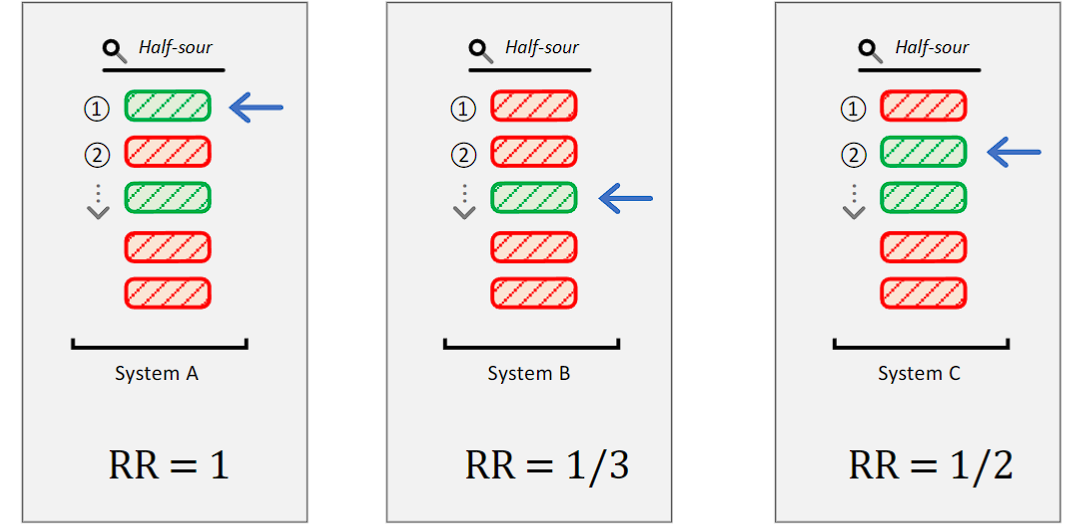
\includegraphics[width=1\textwidth]{assets/pics/rr.png}
            \captionsource{Ilustrasi \f{reciprocal rank} (RR). Kotak berwarnakan hijau menunjukkan teks yang relevan dengan kueri $q$ dan kotak berwarna merah menunjukkan teks yang tidak relevan dengan kueri $q$. Nilai RR pada sistem A, B, dan C berturut-turut adalah 1, 0.33, dan 0.5 karena posisi dari teks yang relevan pertama adalah 1, 3, dan 2.}{\citep{irlecture}.}
            \label{fig:reciprocal-rank}
        \end{figure}
        Metrik lainnya yang sering digunakan untuk mengukur performa sistem pemeringkatan adalah \f{reciprocal rank} (RR). Metrik RR menitikberatkan pada peringkat dari teks relevan pertama dengan kueri $q$. \equ~\ref{eq:reciprocal-rank-start} hingga \equ~\ref{eq:reciprocal-rank-end} menunjukkan cara menghitung RR dari suatu kueri $q$ dan barisan $k$ teks yang diambil oleh sistem.
        \begin{align}
            \text{RR}(q, D_k)\text{@k} &= \begin{cases}
                \label{eq:reciprocal-rank-start}
                \frac{1}{\text{FirstRank}(q, D_k)} & \text{jika } \exists d \in D_k \text{ dengan } \text{rel}(q, d) = 1 \\        
                0 & \text{jika } \forall d \in D_k, \text{ rel}(q, d) = 0 \\
                \end{cases} \in [0, 1], \\
                \label{eq:reciprocal-rank-end}
                \text{FirstRank}(q,D_k) &= \text{posisi teks relevan pertama } d\in D_k \text{ dengan } \text{rel}(q, d) = 1.
        \end{align}

        \pic~\ref{fig:reciprocal-rank} mengilustrasikan metrik RR. Pada gambar tersebut, nilai RR dari sistem A adalah 1 $(\frac{1}{1})$ karena posisi dari teks yang relevan pertama adalah 1. Nilai RR dari sistem B dan sistem C masing-masing adalah  0.33 $(\frac{1}{3})$ dan 0.5 $(\frac{1}{2})$ karena posisi dari teks yang relevan pertama adalah 3 dan 2. Selain itu, jika tidak terdapat teks yang relevan dengan kueri $q$ pada $D_k$, nilai RR dari sistem tersebut adalah 0. 

    \subsubsection{\f{Normalized Discounted Cumulative Gain} (nDCG)}

        \begin{figure}[!ht]
            \centering
            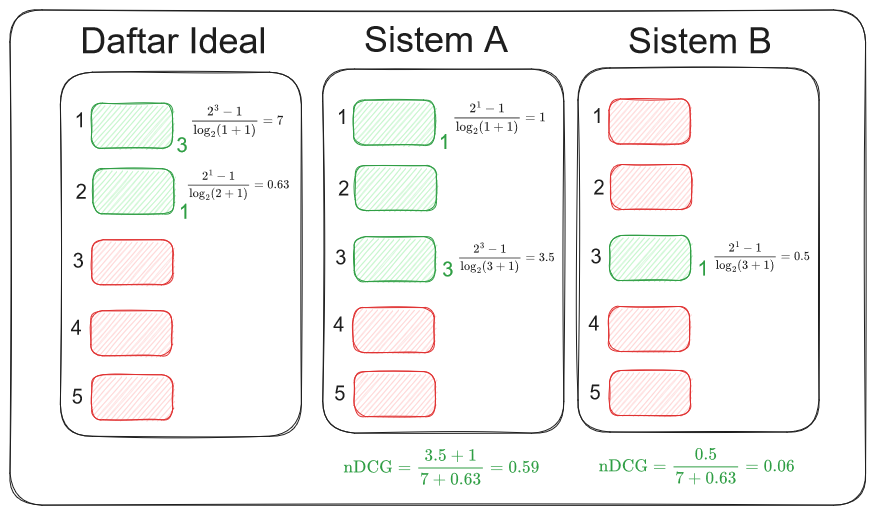
\includegraphics[width=1\textwidth]{assets/pics/contohnDCG.png}
            \captionsource{Ilustrasi perhitungan NDCG. Kotak berwarna hijau menunjukkan teks yang relevan dengan kueri $q$ dan kotak berwarna merah menunjukkan teks yang tidak relevan dengan kueri $q$ serta nilai disebelah kotak berwarnakan hijau menunjukkan \f{judgements} $r$. Nilai NDCG dari sistem A, B, adalah rasio antara DCG dari sistem tersebut dengan DCG dari sistem ideal.}{\citep{irlecture}, telah diolah kembali.}
            \label{fig:ndcg}
        \end{figure}
        \f{Normalized Discounted Cumulative Gain} (NDCG) adalah metrik yang umumnya digunakan untuk mengukur kualitas dari pencarian situs web. Tidak seperti metrik yang telah disebutkan sebelumnya, nDCG dirancang untuk suatu $r$ yang tak biner. \equ~\ref{eq:ndcg-start} hingga \equ~\ref{eq:ndcg-end} menunjukkan cara menghitung NDCG dari suatu kueri $q$ dan barisan $k$ teks yang diambil oleh sistem.
        \begin{align}
            \label{eq:ndcg-start}
            \text{nDCG}(q, D_k)\text{@k} &= \frac{\text{DCG}(q, D_k)\text{@k}}{\text{DCG}(q, D_k^{\text{ideal}})\text{@k}} \in [0, 1], \\
            \label{eq:dcg}
            \text{DCG}(q, D_k)\text{@k} &= \sum_{d \in D_k} \frac{2^{\text{rel}(q, d)} - 1}{\log_2(\text{rank}(d, D_k) + 1)}, \\
            \text{rank}(d,D_k) &= \text{Posisi } d \text{ dalam } D_k, \\
            \text{rel}(q, d) &= r.
            \label{eq:ndcg-end}
        \end{align}

        Perhitungan \f{discounted cumulative gain} (DCG) pada \equ~\ref{eq:dcg} dapat dijelaskan menjadi dua faktor berikut:
        \begin{enumerate}
            \item Faktor $2^{\text{rel}(q, d)} - 1$ menunjukkan bahwa teks yang lebih relevan akan memiliki nilai yang lebih tinggi dari teks yang kurang relevan untuk posisi teks yang sama.
            \item Faktor $\frac{1}{\log_2(\text{rank}(d, D_k) + 1)}$ menunjukkan bahwa teks yang relevan yang muncul pada peringkat tinggi akan memiliki nilai yang lebih besar dari teks dengan relevansi yang sama, tetapi muncul peringkat rendah.
        \end{enumerate}

        Nilai dari NDCG pada \equ~\ref{eq:ndcg-start} adalah nilai DCG pada barisan teks $D_k$ yang dinormalisasi oleh nilai DCG pada barisan teks ideal $D_k^{\text{ideal}}$. Barisan teks ideal $D_k^{\text{ideal}}$ adalah barisan teks yang diurutkan berdasarkan relevansinya dengan kueri $q$.


\section{Pemeringkatan Teks dengan Statistik}
        Untuk mengambil $k$ teks dari kumpulan $\mathcal{D}$ diperlukan suatu fungsi skor $\text{score}(q, d, \mathcal{D})$ yang mengukur relevansi antara kueri $q$ dan teks $d$. Dengan mencari skor antara $q$ terhadap semua teks pada $\mathcal{D}$, barisan teks $D_k = (d_{i_1}, d_{i_2},\dots, d_{i_k})$ dipilih sehingga $\text{score}(q, d_{i_1},\mathcal{D}) \geq \text{score}(q, d_{i_2}, \mathcal{D}) \geq \dots \geq \text{score}(q, d_{i_k},\mathcal{D})$ adalah $k$ teks dengan skor tertinggi.
        Bagian ini menjelaskan dua fungsi skor statistik sederhana yang menjadi \f{baseline} ketika membandingkan performa dari model pemeringkatan teks yang lebih kompleks. \sect~\ref{sec:tfidf} menjelaskan fungsi skor statistik yang berdasarkan pada frekuensi kemunculan kata dan tingkat \f{rarity} kata dalam kumpulan teks. Selanjutnya, \sect~\ref{sec:bm25} membahas fungsi skor statistik yang menjadi \f{baseline} dalam penelitian ini.
    \subsection{\f{Term Frequency - Inverse Document Frequency} (TF-IDF)}
    \label{sec:tfidf}
 
    Fungsi skor TF-IDF adalah fungsi skor statistik yang menghitung $\text{score}(q,d,\mathcal{D})$ antara kueri $q$ dan teks $d$ dengan menghitung frekuensi kemunculan kata dan tingkat \f{rarity} kata. Untuk suatu kueri $q$, misalkan $T_q= \{t_1, t_2, \dots, t_{L_1}\}$ adalah himpunan kata yang terdapat pada kueri $q$. Misalkan juga $T_d = \{t_1, t_2, \dots, t_n\}$ adalah himpunan kata yang terdapat pada teks $d$. Nilai skor antara $q$ dan $d$ diberikan oleh persamaan \equ~\ref{eq:tfidf-start} sampai \equ~\ref{eq:tfidf-end}.
    \begin{align}
        \label{eq:tfidf-start}
        \text{score}(q,d,\mathcal{D}) &= \sum_{t \in T_q \cap T_d} \text{TF-IDF}(t, d, \mathcal{D}) \\
        \label{eq:tf-idf-weight}
        \text{TF-IDF}(t, d, \mathcal{D}) &= \text{tf}(t, d) \times \text{idf}(t, \mathcal{D}) \\
        \text{tf}(t, d) &= \frac{\text{Count}(t, d)}{|d|} \\
        \text{Count}(t, d) &= \text{jumlah kemunculan } t \text{ dalam } d \\
        \text{idf}(t, \mathcal{D}) &= \begin{cases}
            \log_2\left(\frac{|\mathcal{D}|}{\text{df}(t, \mathcal{D})}\right) & \text{jika } \text{df}(t, \mathcal{D}) > 0 \\
            0 & \text{jika } \text{df}(t, \mathcal{D}) = 0
        \end{cases} \\
        \text{df}(t, \mathcal{D}) &= \text{jumlah teks pada } \mathcal{D} \text{ yang mengandung } t
        \label{eq:tfidf-end}
    \end{align}

    Skor untuk pasangan $(q,d)$ dihitung dengan menjumlahkan skor TF-IDF dari setiap kata yang terdapat pada kueri $q$ dan teks $d$. skor TF-IDF dari suatu kata $t$ adalah perkalian antara \f{term frequency} $\text{tf}(q,d)$ dan \f{inverse document frequency} $\text{idf}(t,\mathcal{D})$. Fungsi skor pada \equ~\ref{eq:tfidf-start} dapat dijelaskan menjadi dua faktor utama berikut:
    \begin{enumerate}
        \item Faktor $\text{tf}(t, d)$ menunjukkan bahwa nilai TF-IDF meningkat seiring dengan bertambahnya frekuensi kemunculan kata $t$ pada teks $d$.
        \item Faktor $\text{idf}(t, \mathcal{D})$ menunjukkan bahwa nilai TF-IDF meningkat seiring dengan \textit{rarity} dari kata $t$ pada himpunan teks $\mathcal{D}$. Akibatnya, kata yang jarang muncul pada himpunan teks $\mathcal{D}$ yang muncul pada suatu teks tertentu akan menghasilkan skor yang tinggi. Sementara itu, kata-kata yang sering muncul pada koleksi teks $\mathcal{D}$ memiliki nilai \textit{downgraded}. \pic~\ref{fig:idf-graph} menunjukkan grafik dari fungsi $\text{idf}$.
    \end{enumerate}
    \begin{figure}[!ht]
    \centering
    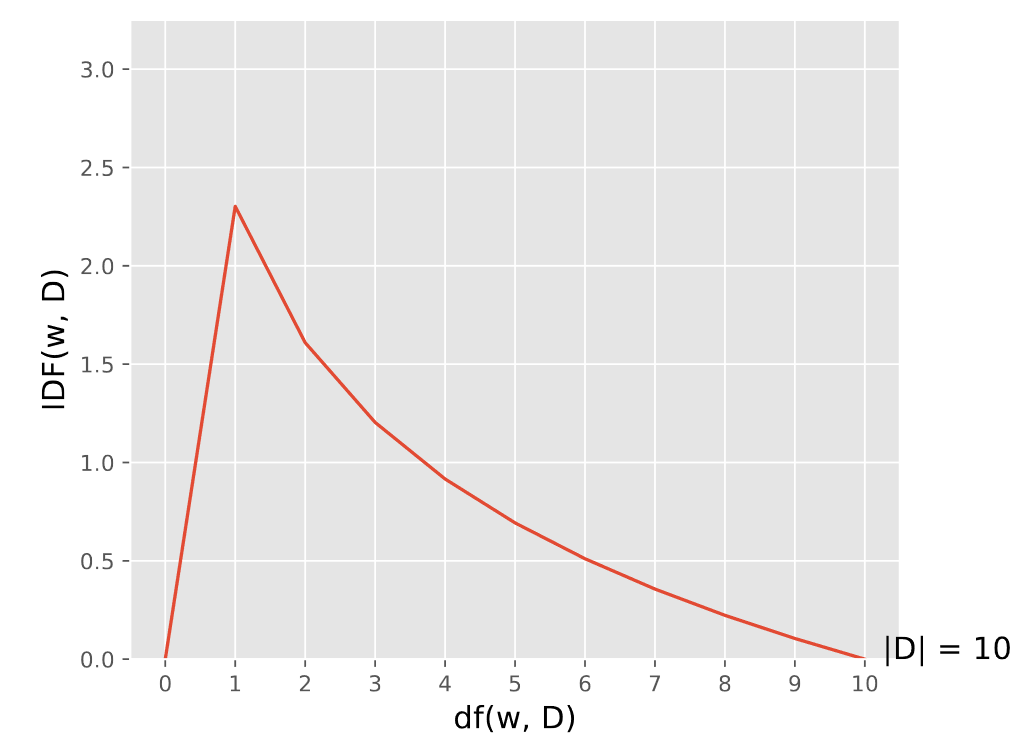
\includegraphics[width=0.75\textwidth]{assets/pics/idf-graph.png}
        \captionsource{Grafik dari fungsi $\text{idf}$. Nilai idf menurun seiring dengan bertambahnya nilai $\text{df}(t, \mathcal{D})$.}{\citep{stanfordir}.}
        \label{fig:idf-graph}
    \end{figure}

    Kata-kata seperti preposisi atau kata ganti akan menghasilkan skor TF-IDF yang sangat rendah. Hal ini menyiratkan bahwa kata-kata tersebut memiliki sedikit relevansi dalam teks dan bisa diabaikan. Di sisi lain, kata-kata yang muncul secara berlebihan dalam satu teks tetapi jarang muncul dalam teks lainnya akan menghasilkan nilai $\text{tf}(t, d)$ dan $\log \left(\frac{\mathcal{D}}{\text{df}(t, \mathcal{D})}\right)$ yang relatif besar. Dampaknya adalah skor TF-IDF yang dihasilkan juga menjadi signifikan. \pic~\ref{fig:tf-idf-matriks} menunjukkan contoh perhitungan skor TF-IDF untuk suatu kumpulan teks.

    
    \begin{figure}[!ht]
        \centering
        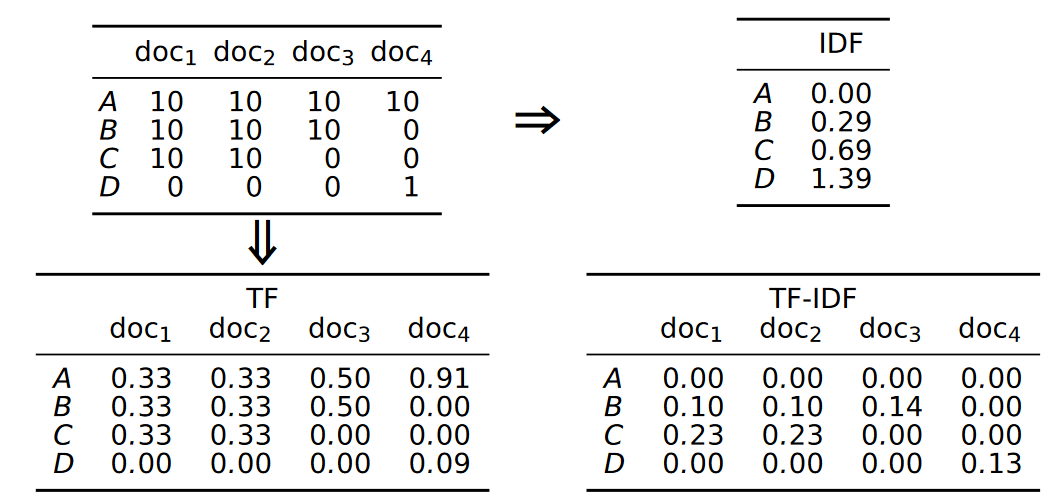
\includegraphics[width=1\textwidth]{assets/pics/tf-idf-matriks.png}
        \captionsource{Ilustrasi perhitungan skor TF-IDF untuk suatu kumpulan teks.}{\citep{stanfordir}.}
        \label{fig:tf-idf-matriks}
    \end{figure}
    \subsection{\f{Best Match 25} (BM25)}
    \label{sec:bm25}
    
    BM25 (\f{Best Match attempt} 25)  merupakan pengembangan dari fungsi skor TF-IDF dengan perbedaan utama pada fungsi nilai yang berkaitan dengan frekuensi kata -- digunakan $\text{score}_{\text{BM25}}(q,d)$ (\equ~\ref{eq:bm25-weight}) daripada $\text{tf}(q,d)$ (\equ~\ref{eq:tf-idf-weight}). Pada fungsi $\text{score}_{\text{BM25}(q,d)}$ terdapat 2 parameter yang dapat diatur, yaitu $b$, dan $k_1$. Setiap parameter mempunyai efek yang berbeda terhadap nilai $\text{score}_{\text{BM25}(q,d)}$ yang dihasilkan. Sebelum menjelaskan efek dari setiap parameter, \equ~\ref{eq:bm25scoring} hingga \equ~\ref{eq:bm25-end} menunjukkan cara menghitung skor relevansi dari suatu kueri $q$ dan teks $d$. 
    \begin{align}
        \label{eq:bm25scoring}
        \text{score}(q,d,\mathcal{D}) &= \sum_{t \in T_q \cap T_d} \text{BM25}(t, d, \mathcal{D}),\\
        \label{eq:bm25-weight}
        \text{BM25}(t, d, \mathcal{D}) &= \text{idf}_{\text{BM25}}(t, \mathcal{D}) \times \text{score}_{\text{BM25}}(q,d,\mathcal{D}), \\
        \text{score}_{\text{BM25}}(t,d) &= \frac{\text{tf}(t, d) \times (k_1 + 1)}{\text{tf}(t, d) + k_1 \times (1 - b + b \times \frac{|d|}{\text{avgdl}})}, \\
        \label{eq:smoothed-idf}
        \text{idf}_{\text{BM25}}(t, \mathcal{D}) &= \log\left(1+\frac{|\mathcal{D}| - \text{df}(t, \mathcal{D}) + 0.5}{\text{df}(t, \mathcal{D}) + 0.5}\right), \\
        \text{avgdl} &= \text{rata-rata panjang teks pada koleksi } \mathcal{D}.
        \label{eq:bm25-end}
    \end{align}
    Efek dari masing-masing parameter dan faktor pada $\text{score}_{\text{BM25}}(t,d)$ dapat dijelaskan sebagai berikut:
    \begin{enumerate}
        \item Faktor $\frac{|\text{d}|}{\text{avgdl}}$ pada $\frac{\text{tf}(t, d) \times (k_1 + 1)}{\text{tf}(t, d) + k_1 \times \left(1 - b + b \times \textcolor{black}{\frac{|d|}{\text{avgdl}}}\right)}$ men-\f{penalize} skor pada teks yang panjangnya lebih besar dari rata-rata panjang teks pada himpunan teks $\mathcal{D}$. \pic~\ref{fig:effect-bm25-long-doc} menjukkan efek dari perbedaan nilai $\text{avgdl}$ terhadap skor yang dihasilkan, makin besar rasio $\frac{|d|}{\text{avgdl}}$ makin kecil skor yang dihasilkan.
        \item Nilai $b$ menentukan seberapa besar efek dari faktor $\frac{|d|}{\text{avgdl}}$ terhadap skor yang dihasilkan. \pic~\ref{fig:effect-bm25-param-b} menunjukkan efek dari perbedaan nilai $b$ terhadap skor yang dihasilkan. Untuk $\frac{|d|}{\text{avgdl}}=1$, faktor $b$ tidak memiliki pengaruh terhadap skor. Nilai $b$ yang umum dipilih berada pada rentang $[0.5, 0.8]$ \citep{irlecture}.
        \item  Nilai $k_1$ men-\f{penalize} kemunculan kata $t$ pada teks $d$ yang berlebih. \pic~\ref{fig:effect-bm25-param-k} menunjukkan efek dari perbedaan nilai $k_1$ terhadap skor yang dihasilkan. untuk nilai $k_1$ yang ekstrim, nilai $\text{score}_{\text{BM25}}(t,d)$ hanya menjadi indikator saja dari kemunculan kata $t$ pada teks $d$. Nilai $k_1$ yang umum dipilih berada pada rentang $[1.2, 2.0]$ \citep{irlecture}.
    \end{enumerate}
    \begin{figure}[!ht]
        \centering
        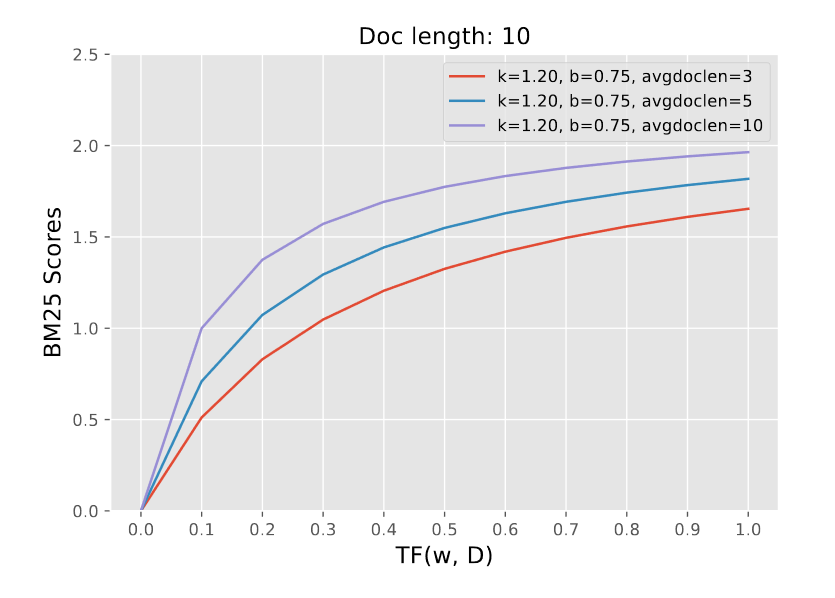
\includegraphics[width=0.75\textwidth]{assets/pics/effect-bm25-long-doc.png}
        \captionsource{Kumpulan grafik dari fungsi $\text{score}_{\text{BM25}}(t,d)$ dengan perbedaan nilai $\text{avgdl}$.}{\citep{stanfordir}.}
        \label{fig:effect-bm25-long-doc}
    \end{figure}

    \begin{figure}[!ht]
        \centering
        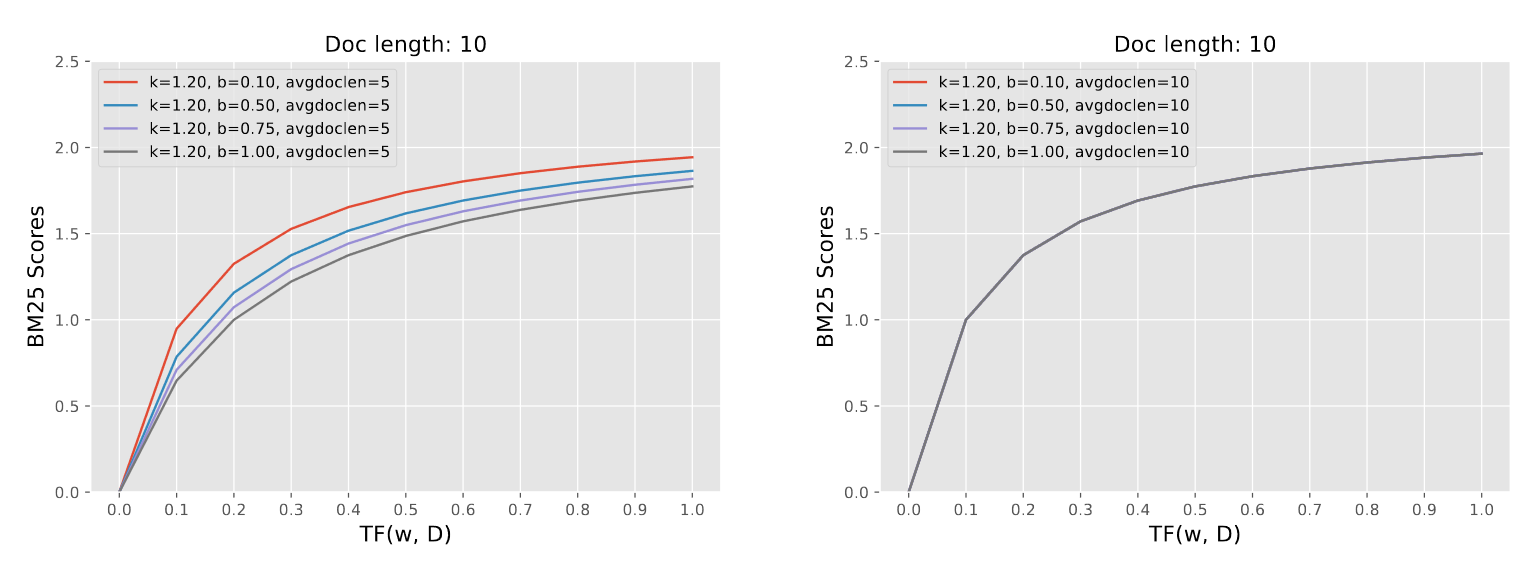
\includegraphics[width=1\textwidth]{assets/pics/effect-bm25-param-b.png}
        \captionsource{Kumpulan grafik dari fungsi $\text{score}_{\text{BM25}}(t,d)$ dengan perbedaan nilai $b$.}{\citep{stanfordir}.}
        \label{fig:effect-bm25-param-b}
    \end{figure}
    \begin{figure}[!ht]
        \centering
        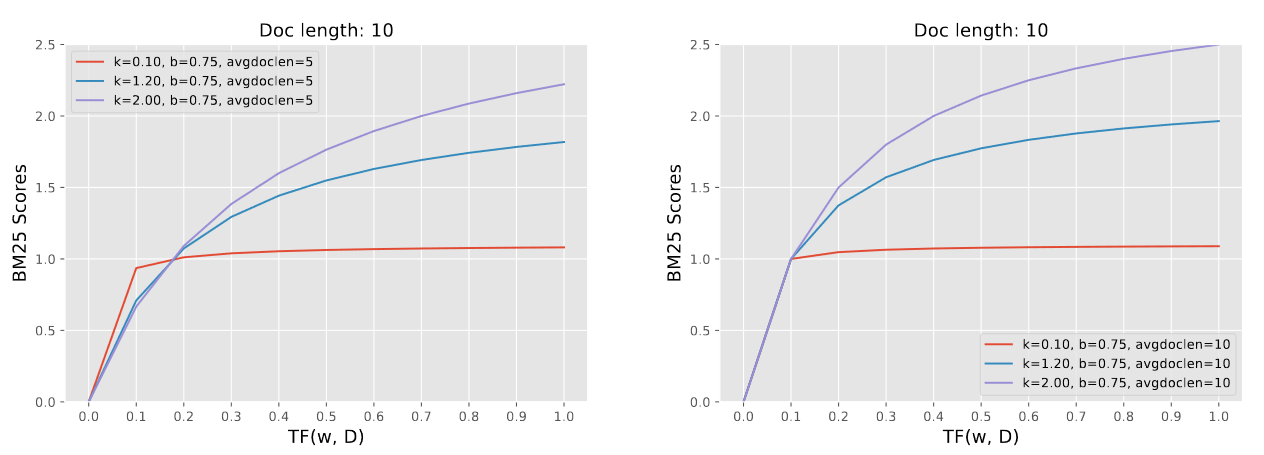
\includegraphics[width=1\textwidth]{assets/pics/effect-bm25-param-k.png}
        \captionsource{Kumpulan grafik dari fungsi $\text{score}_{\text{BM25}}(t,d)$ dengan perbedaan nilai $k_1$.}{\citep{stanfordir}.}
        \label{fig:effect-bm25-param-k}
    \end{figure}
    
    Perbedaan \f{minor} lainnya ada pada fungsi $\text{idf}$. Fungsi $\text{idf}$ pada BM25 merupakan versi \f{smoothing} dari $\text{idf}$ dengan tujuan untuk menghindari nilai $\text{idf}$ yang bernilai 0 ketika kata $t$ tidak muncul pada himpunan teks $\mathcal{D}$ -- semata-mata untuk konsistensi dengan asumsi bahwa kata $t$ yang tidak muncul pada himpunan teks $\mathcal{D}$ memiliki nilai $\text{idf}$ (\f{rarity}) yang paling tinggi. \pic~\ref{fig:smoothed-idf} menunjukkan perbedaan antara $\text{idf}_{BM25}$ dan $\text{idf}$. Perbedaan utamanya terjadi ketika $\text{df}(t,\mathcal{D}) = 0$, nilai dari  $\text{idf}_{BM25}$ tak nol dan mengikuti pola yang diharapkan. Ketika $\text{df}(t,\mathcal{D})>0$, nilai dari $\text{idf}_{\text{BM25}}$ dan $\text{idf}$ hampir serupa.

    \begin{figure}[!ht]
        \centering
        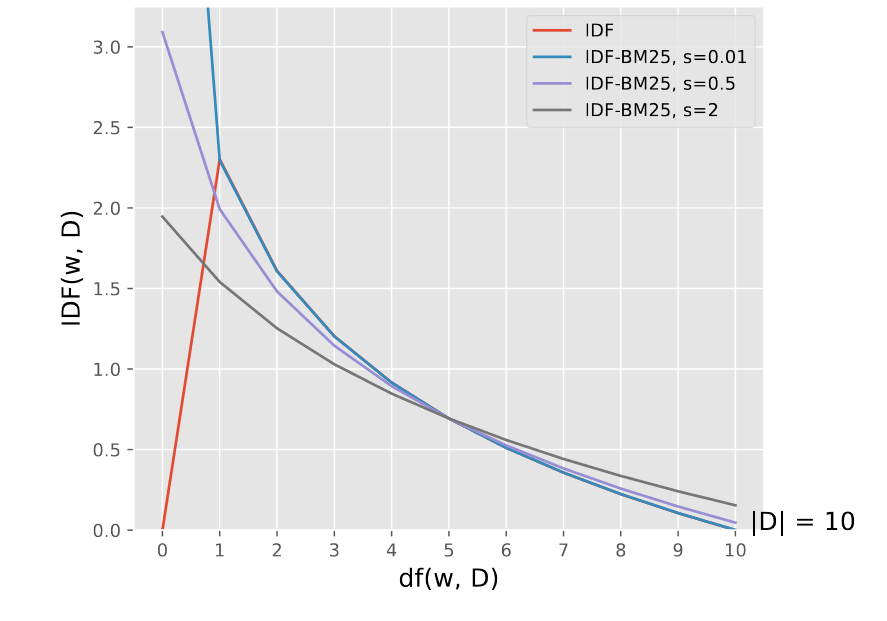
\includegraphics[width=0.75\textwidth]{assets/pics/smoothed-idf.png}
        \captionsource{Perbedaan antara $\text{idf}_{\text{BM25}}$ dan $\text{idf}$.}{\citep{stanfordir}.}
        \label{fig:smoothed-idf}
    \end{figure}


\section{\f{Deep Learning}}
    \begin{figure}[!ht]
        \centering
        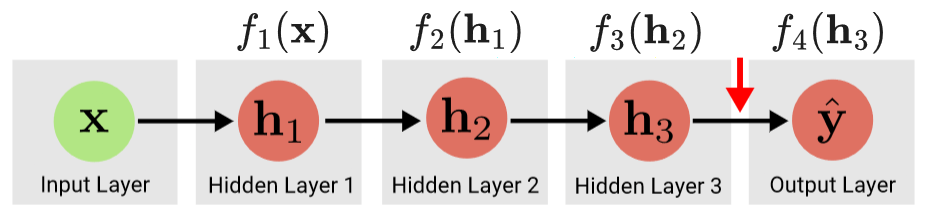
\includegraphics[width=0.50\textwidth]{assets/pics/dag-dl.png}
        \captionsource{Ilustrasi dari \f{Directed Acyclic Graph} (DAG) pada arsitektur \f{deep learning feed-forward neural network} (FFN).}{\citep{geiger2022deeplearning}, telah diolah kembali.}
        \label{fig:deep-learning-FFN-dag}
    \end{figure}
    Arsitektur \f{deep learning} merujuk pada model \f{machine learning} yang tersusun dari fungsi-fungsi terturunkan (yang biasa disebut sebagai \f{layer}), dimana komposisi antara fungsi-fungsi tersebut dapat digambarkan sebagai \f{directed acyclic graph} (DAG) yang memetakan suatu \f{input} ke suatu \f{output}. Biasanya, setiap fungsi dalam Arsitektur \f{deep learning} memiliki parameter yang ingin diestimasi atau dicari dengan data.
    
    \pic~\ref{fig:deep-learning-FFN-dag} menunjukkan arsitektur \f{deep learning} yang sederhana, yaitu \f{feed-forward neural network} (FFN). Pada \pic~\ref{fig:deep-learning-FFN-dag}, \f{input} $\mathbf{x}$ akan dipetakan ke \f{output} $\mathbf{\hat y}$ melalui serangkaian fungsi $f_1, f_2, f_3,f_4$ yang disebut sebagai \f{layer}. Setiap \f{layer} $f_i$ memiliki parameter $\theta_i$ yang akan diestimasi dengan data. Selain itu, \f{output} dari \f{layer} $f_i$ akan menjadi \f{input} dari \f{layer} $f_{i+1}$. \f{Output} dari \f{layer} $f_4$ adalah \f{output} dari model. Model pada \pic~\ref{fig:deep-learning-FFN-dag} dapat ditulis sebagai \equ~\ref{eq:deep-learning-FFN-dag}.
    \begin{align}
        \label{eq:deep-learning-FFN-dag}
        \mathbf{\hat y} = f_{\text{model}}(\mathbf{x}; \bm{\theta}) &= f_4(f_3(f_2(f_1(\mathbf{x}; \bm{\theta}_1); \bm{\theta}_2); \bm{\theta}_3); \bm{\theta}_4),
    \end{align}
    dengan $\bm{\theta} = \{\bm{\theta}_1, \bm{\theta}_2, \bm{\theta}_3, \bm{\theta}_4\}$ adalah parameter dari model.

    \subsection{\f{Multilayer Perceptron} (MLP)}

    \f{Multi-layer perceptron} (MLP) adalah \f{feed-forward neural network} dengan setiap fungsi $f_i$ adalah fungsi linear yang diikuti oleh fungsi aktivasi non-linear $\phi$  yang diterapkan \f{element-wise} pada setiap \f{output}-nya. \f{Hyperparameter} (parameter yang dipilih prior proses pelatihan dilakukan) lainnya selain fungsi aktivasi adalah kedalamaan model $L$, dan dimensi \f{output} dari setiap \f{layer} $d_1, d_2, \dots, d_L$.

    Untuk permasalahan regresi dengan \f{input} $\mathbf{x}\in \mathbb{R}^{d_0}$ dan \f{output} $\mathbf{y} \in \mathbb{R}^{d_L}$, \equ~\ref{eq:FFN-regesi-start} hingga \equ~\ref{eq:FFN-regesi-end} menunjukkan arsitektur MLP untuk permasalahan regresi dengan $L$ \f{layer} dan fungsi aktivasi $\phi$.
    \begin{align}
        \label{eq:FFN-regesi-start}
        f_{\text{model}}(\mathbf{x};\bm{\theta}) &= f_L(f_{L-1}(\dots f_1(\mathbf{x})) \dots), \\
        f_L(\mathbf{x}) &= \mathbf{x} \mathbf{W}_L + \mathbf{b}_L \in \mathbb{R}^{d_L}, \\
        f_l(\mathbf{x};\mathbf{W}_l, \mathbf{b_l}) &= \phi( \mathbf{x} \mathbf{W}_l + \mathbf{b}_l) \in \mathbb{R}^{d_l}, \quad l = 1, 2, \dots, L-1,
        \label{eq:FFN-regesi-end}
    \end{align} 
    dengan keterangan sebagai berikut:
    \begin{flalign*}
        \phi(\mathbf{x}) &= \text{fungsi aktivitasi non-linear},&& \\
        \bm{\theta} &= \{\mathbf{W}_1, \mathbf{b}_1, \mathbf{W}_2, \mathbf{b}_2, \dots, \mathbf{W}_L, \mathbf{b}_L\},&& \\
        \mathbf{W}_l &= \text{matriks bobot}  \in \mathbb{R}^{d_{l-1} \times d_l},&& \\
        \mathbf{b}_l &= \text{vektor bias} \in \mathbb{R}^{d_l}.&&
    \end{flalign*}

    Untuk Permasalahan Klasifikasi Biner dengan \f{input} $\mathbf{x}\in \mathbb{R}^{d_0}$ dan \f{output} $y \in \{0, 1\}$, \equ~\ref{eq:FFN-klasifikasi-biner-start} hingga \equ~\ref{eq:FFN-klasifikasi-biner-end} menunjukkan arsitektur MLP untuk permasalahan klasifikasi biner.
    \begin{align}
        \label{eq:FFN-klasifikasi-biner-start}
        f_{\text{model}}(\mathbf{x};\bm{\theta}) &= f_L(f_{L-1}(\dots f_1(\mathbf{x})) \dots), \\
        f_L(\mathbf{x}) &= \sigma(\mathbf{x} \mathbf{W}_L + \mathbf{b}_L), \\
        \sigma(x) &= \frac{1}{1 + e^{x}} \in (0, 1), \\
        \text{decision}(\mathbf{x};\bm{\theta}) &= \begin{cases}
        1 & \text{jika } f_{\text{model}}(\mathbf{x};\bm{\theta}) \geq \text{threshold} \\
        0 & \text{jika } f_{\text{model}}(\mathbf{x};\bm{\theta}) < \text{threshold},
        \end{cases} \\
        \label{eq:FFN-klasifikasi-biner-end}
        \text{threshold}&\in [0, 1].
    \end{align}

    Perbedaan utama antara MLP untuk permasalahan regresi dan klasifikasi adalah fungsi aktivasi pada \f{output layer}. Pada permasalahan regresi, fungsi aktivasi pada \f{output layer} adalah fungsi identitas, sedangkan pada permasalahan klasifikasi, fungsi aktivasi pada \f{output layer} adalah fungsi \f{sigmoid}. Tujuan pengunaan fungsi \f{sigmoid} pada permasalahan klasifikasi adalah untuk memastikan bahwa \f{output} dari model berada pada rentang $[0, 1]$, nilai tersebut dapat diinterpretasikan sebagai probabilitas $\mathbf{x}$ termasuk pada kelas positif. Selain itu, \f{threshold} pada \equ~\ref{eq:FFN-klasifikasi-biner-end} digunakan untuk menentukan kelas dari $\mathbf{x}$.

    \subsection{Fungsi Aktivasi}

    Fungsi aktivasi pada setiap fungsi $f_i$ pada \f{multilayer perceptron} digunakan untuk menambahkan non-linearitas pada model. Sebab, tanpa adanya fungsi aktivasi non-linear, model \f{multilayer perceptron} akan menjadi model linear. Selain itu, fungsi aktivasi juga biasanya adalah fungsi yang terturunkan, meskipun tidak perlu terturunkan disetiap titik. \tab~\ref{tab:activation-function} menunjukkan beberapa fungsi aktivasi yang sering digunakan pada \f{multilayer perceptron}. \pic~\ref{fig:activation-function} menunjukkan grafik dari fungsi aktivasi pada \tab~\ref{tab:activation-function} dan turunannya.
    \begin{table}[!ht]
        \centering
        \caption{Beberapa fungsi aktivasi yang sering digunakan pada \f{multilayer perceptron}.}
        \label{tab:activation-function}
        \begin{tabular}{|c|c|}
            \hline
            \textbf{Fungsi Aktivasi} & \textbf{Persamaan} \\
            \hline
            \hline
            Sigmoid & $\sigma(x) = \frac{1}{1 + e^{-x}}$ \\
            \hline
            Tanh & $\tanh(x) = \frac{e^x - e^{-x}}{e^x + e^{-x}}$ \\
            \hline
            ReLU & $\text{ReLU}(x) = \max(0, x)$ \\
            \hline
            Leaky ReLU & $\text{LeakyReLU}(x) = \max(\alpha x, x), \alpha \in [0, 1]$ \\
            \hline
        \end{tabular}
    \end{table}
    \begin{figure}[!ht]
        \centering
        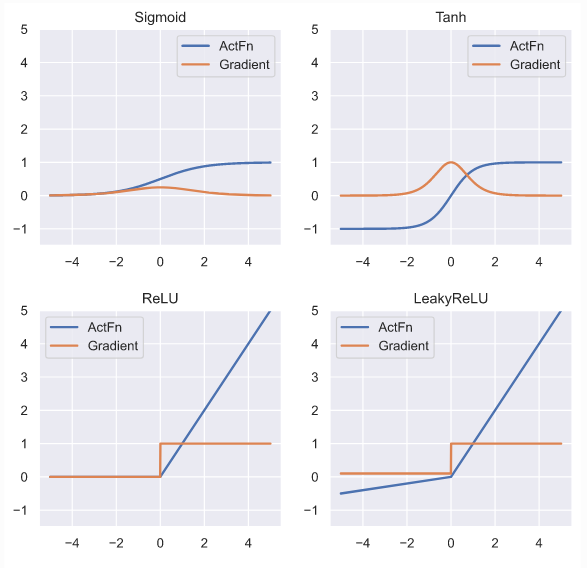
\includegraphics[width=0.5\textwidth]{assets/pics/act_function.png}
        \captionsource{Grafik dari fungsi aktivasi pada \tab~\ref{tab:activation-function} dan turunannya.}{\citep{uvadlc}.}
        \label{fig:activation-function}
    \end{figure}


    \subsection{Fungsi \f{Loss}}
    Misalkan $\mathcal{D} = \{(\mathbf{x}_1, y_1), (\mathbf{x}_2, y_2), \dots, (\mathbf{x}_n, y_n)\}$ adalah \f{dataset} yang terdiri dari $n$ pasangan \f{input} dan \f{output}. Parameter $\bm{\theta}$ pada $f_{\text{model}}$ diestimasi dengan melakukan \f{fitting} pada \f{dataset} $\mathcal{D}$. Untuk melakukan \f{fitting} pada \f{dataset} $\mathcal{D}$, diperlukan suatu fungsi \f{loss} yang mengukur seberapa baik hasil pemetaan $f_{\text{model}}$ pada \f{input} $\mathbf{x}_i$ terhadap \f{output} $\mathbf{y}_i$. Meskipun sembarang fungsi yang terturunkan dapat digunakan sebagai fungsi \f{loss}, namun pemilihan fungsi \f{loss} berdasarkan \f{maximum likelihood estimation} (MLE) lebih disarankan. 
    
    Untuk permasalahan klasifikasi biner, fungsi \f{loss} yang sering digunakan adalah \f{binary cross entropy} (BCE) seperti yang ditinjukkan pada \equ~\ref{eq:bce}. Penurunan fungsi \f{loss} BCE dengan mengikuti prinsip MLE yang akan dijelaskan pada bagian berikut.
    
    Misalkan $y_i \mid \mathbf{x}$ mengikuti distribusi bernoulli dengan parameter $\text{p} = f_{\text{model}}(\mathbf{x};\bm{\theta})$ yang saling independen antara satu sama lainnya. \equ~\ref{eq:definisi-random-variable} menunjukkan definisi dari $y_i \mid \mathbf{x}$.
    \begin{align}
        \label{eq:definisi-random-variable}
        y_i \mid \mathbf{x} &\overset{\text{iid}}{\sim} \text{Bernoulli}(f_{\text{model}}(\mathbf{x};\bm{\theta})), \\
        p(y_i \mid \mathbf{x}) &= f_{\text{model}}(\mathbf{x};\bm{\theta})^{y_i} (1 - f_{\text{model}}(\mathbf{x};\bm{\theta}))^{1 - y_i}.
    \end{align} 

    Fungsi $\f{likelihood}$ dari $\bm{\theta}$ terhadap \f{dataset} $\mathcal{D}$ dapat ditulis sebagai berikut:
    \begin{align}
        \mathcal{L}(\bm{\theta}) &= \prod_{i=1}^N p(y_i \mid \mathbf{x}_i; \bm{\theta}).
    \end{align}

    Dengan prinsip MLE, parameter $\bm{\theta}$ yang dicari adalah parameter $\bm{\theta}$ yang memaksimalkan fungsi \f{likelihood} $\mathcal{L}(\bm{\theta})$,
    \begin{align}
        \bm{\theta}_{\text{MLE}} &= \arg\max_{\bm{\theta}} \mathcal{L}(\bm{\theta}).
    \end{align}

    Untuk mempermudah perhitungan, fungsi \f{likelihood} diubah menjadi negatif \f{log-likelihood} $\mathcal{\ell}(\bm{\theta})$, sehingga permasalahan optimasi dapat ditulis seperti \equ~\ref{eq:log-likelihood} hingga \equ~\ref{eq:log-likelihood-end}.
    \begin{align}
        \label{eq:log-likelihood}
        \ell{(\bm{\theta})} &= -\log\mathcal{L}(\bm{\theta}), \\
        &= -\sum_{i=1}^N \log\left(p(y_i \mid \mathbf{x}_i; \bm{\theta})\right), \\
        \label{eq:log-likelihood-end}
        \bm{\theta}_{\text{MLE}} &= \arg\min_{\bm{\theta}} \ell(\bm{\theta}).
    \end{align} 

    Dengan mengganti $p(y_i \mid \mathbf{x}_i; \bm{\theta})$ dengan fungsi distribusi-nya, maka fungsi \f{loss} yang digunakan untuk permasalahan klasifikasi biner adalah \f{binary cross entropy} (BCE) seperti pada \equ~\ref{eq:bce}. \pic~\ref{fig:dl-training-graph-dag} mengilustrasikan \f{directed acyclic graph} (DAG) dari model ketika proses pelatihan dilakukan.
    \begin{align}
        \bm{\theta}_{\text{MLE}} &= \arg\min_{\bm{\theta}}\sum_{i=1}^{N}\underbrace{-y_i \log\left(f_{\text{model}}(\mathbf{x}_i; \bm{\theta})\right) - (1 - y_i) \log\left(1 - f_{\text{model}}(\mathbf{x}_i; \bm{\theta})\right)}_{\text{Binary Cross Entropy Loss } L(y_i, f_{\text{model}}(\mathbf{x}_i; \bm{\theta}))}, \\
        \label{eq:bce} 
        L(y_i, f_{\text{model}}(\mathbf{x}_i; \bm{\theta})) &= -y_i \log\left(f_{\text{model}}(\mathbf{x}_i; \bm{\theta})\right) - (1 - y_i) \log\left(1 - f_{\text{model}}(\mathbf{x}_i; \bm{\theta})\right).
    \end{align}
    \begin{figure}[!ht]
        \centering
        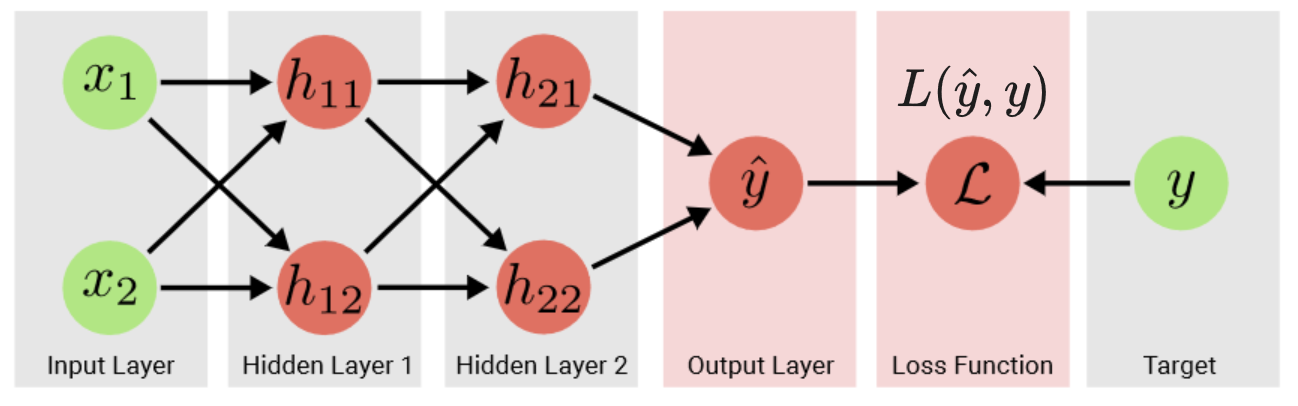
\includegraphics[width=1\textwidth]{assets/pics/dl-training-graph.png}
        \captionsource{Ilustrasi dari \f{Directed Acyclic Graph} (DAG) pada model \f{deep learning} ketika proses pelatihan dilakukan.}{\citep{geiger2022deeplearning}, telah diolah kembali.}
        \label{fig:dl-training-graph-dag}
    \end{figure}

    Untuk mendapatkan $f_\text{model}$ dengan performa yang baik, dibutuhkan model dengan nilai $\ell(\bm{\theta})$ seminimum mungkin. Namun, pencarian $\bm{\theta}$ sehingga $ \ell (\bm{\theta})$ minumum secara analitik tidak dapat dilakukan karena non-linearitas yang ada pada model, dengan kata lain solusi dari $\nabla_{\bm{\theta}} \ell(\bm{\theta}) = 0$ tidak dapat dicari secara analitik. Sebagai gantinya, pencarian $\bm{\theta}$ dilakukan secara numerik dengan menggunakan metode \f{gradient descent} yang akan dijelaskan pada bagian selanjutnya.
    
\subsection{\f{Optimasi} Parameter}

    \f{Gradient descent} adalah metode numerik yang digunakan untuk mencari nilai $\bm{\theta}$ yang meminimalkan fungsi \f{loss} $\ell(\bm{\theta})$. Pada metode \f{gradient descent}, nilai $\bm{\theta}$ di-\f{update} secara iteratif dengan mengikuti arah negatif dari \f{gradient} $\nabla_{\bm{\theta}} \ell(\bm{\theta})$ yang menunjukkan arah dari penurunan fungsi \f{loss} $\ell(\bm{\theta})$. Untuk kumpulan data $\mathcal{D} = \{(\mathbf{x}_1, y_1), (\mathbf{x}_2, y_2), \dots, (\mathbf{x}_n, y_n)\}$, \equ~\ref{eq:gradient-descent} menunjukkan algoritma \f{gradient descent} untuk mencari nilai $\bm{\theta}$.
    \begin{align}
        \label{eq:gradient-descent}
        \bm{\theta}^{(t+1)} &= \bm{\theta}^{(t)} - \eta \frac{1}{n} \sum_{i=1}^{n} \nabla_{\bm{\theta}} L(y_i, f_{\text{model}}(\mathbf{x}_i; \bm{\theta}^{(t)})),
    \end{align}
    dengan $\eta \in \mathbb{R}^+$ adalah \f{learning rate} yang menentukan seberapa besar perubahan pada $\bm{\theta}$ pada setiap iterasi.

    Perlu diketahui bahwa pada metode \f{gradient descent} memperbarui parameter dengan mengambil rata-rata \f{gradient} dari semua data pada \f{dataset} pelatihan $\mathcal{D}$. Hal ini menciptakan masalah ketika model menggunakan banyak parameter dan jumlah data pada \f{datasets} latih besar, yaitu komputasi \f{forward pass} dan \f{backward pass} menjadi sangat mahal dan diperlukan memori yang besar untuk menyimpan gradien dari semua data pada \f{dataset} latih. Untuk mengatasi masalah tersebut, digunakan metode \f{stochastic gradient descent} (SGD) dimana setiap \f{update} dari parameter $\bm{\theta}$ dihitung dengan mengambil rata-rata \f{gradient} dari sebagian data pada \f{dataset} $\mathcal{B}\subseteq\mathcal{D}$. \equ~\ref{eq:stochastic-gradient-descent} menunjukkan algoritma \f{stochastic gradient descent}.
    \begin{align}
        \mathcal{B} = \{(\mathbf{x}_{i_1}, y_{i_1}), (\mathbf{x}_{i_2}, y_{i_2}), \dots, (\mathbf{x}_{i_b}, y_{i_b})\} &\subseteq \mathcal{D}, \mid \mathcal{B} \mid \ll \mid \mathcal{D} \mid, \\
        \label{eq:stochastic-gradient-descent-approx}
        \nabla_{\bm{\theta}}{L_\mathcal{B}}(\bm{\theta}) &= 
         \frac{1}{b} \sum_{i=1}^{b} \nabla_{\bm{\theta}} L(y_{i}, f_{\text{model}}(\mathbf{x}_{i}; \bm{\theta})), \\
        \label{eq:stochastic-gradient-descent}
        \bm{\theta}^{(t+1)} &= \bm{\theta}^{(t)} - \eta \nabla_{\bm{\theta}} \mathcal{L_B}(\bm{\theta}^{(t)}).
    \end{align}

    \f{Hyperparameter} \f{learning rate} mengatur laju dari perubahan parameter $\bm{\theta}$ pada setiap iterasi pembaruan. Dengan demikian, pemilihan \f{learning rate} berpengaruh terhadap kekonvergenan optimasi yang dilakukan. Jika \f{learning rate} yang digunakan terlalu kecil, model membutuhkan waktu yang jauh lebih lama untuk mencapai nilai parameter $\bm{\theta}$ yang optimal. Di lain sisi, pemilihan \f{learning rate} yang terlalu besar dapat membuat model tidak dapat menemukan nilai parameter $\bm{\theta}$ yang optimal. \pic~\ref{fig:learning-rate-bad} mengilustrasikan proses pembaruan parameter $\bm{\theta}$ dengan \f{learning rate} yang terlalu kecil dan terlalu besar, dan \pic~\ref{fig:learning-rate-good} mengilustrasikan proses pembaruan parameter $\bm{\theta}$ dengan \f{learning rate} yang baik.
\begin{figure}[!ht]
    \centering
    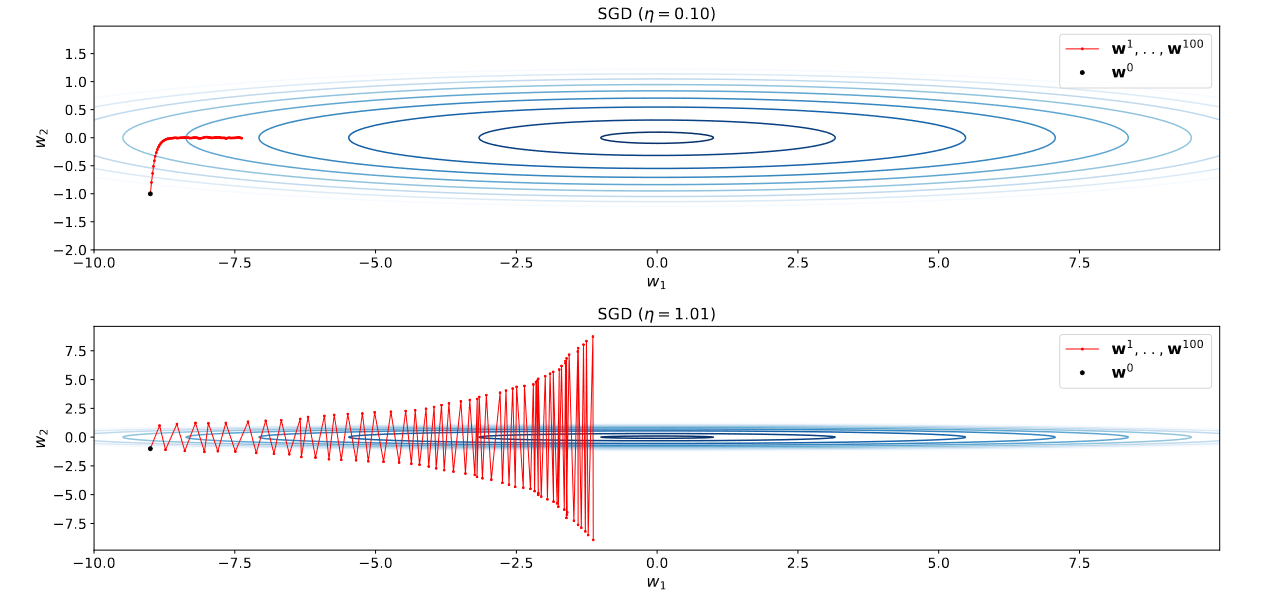
\includegraphics[width=1\textwidth]{assets/pics/learning-rate-bad.png}
    \captionsource{Seratus iterasi pertama dari pembaruan parameter $\bm{\theta} = \{w_1, w_2\}$ dengan \f{learning rate} yang terlalu kecil dan terlalu besar.}{\citep{geiger2022deeplearning}.}
    \label{fig:learning-rate-bad}
\end{figure}

\begin{figure}[!ht]
    \centering
    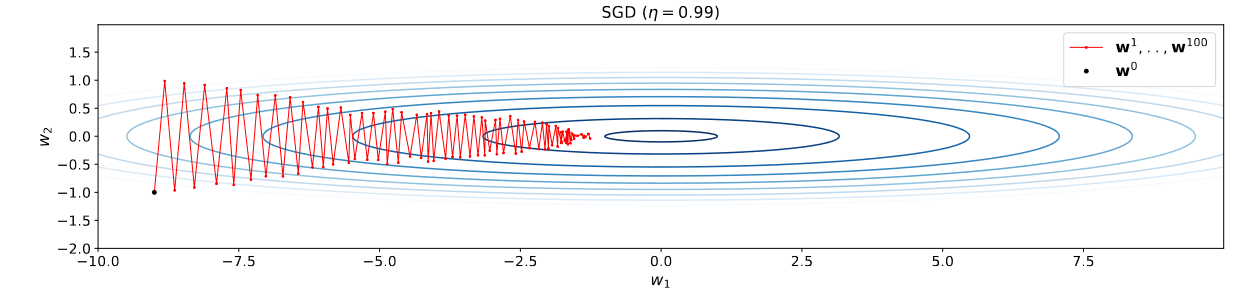
\includegraphics[width=1\textwidth]{assets/pics/learning-rate-good.png}
    \captionsource{Seratus iterasi pertama dari pembaruan parameter $\bm{\theta} = \{w_1, w_2\}$ dengan \f{learning rate} yang baik.}{\citep{geiger2022deeplearning}.}
    \label{fig:learning-rate-good}
\end{figure}

Untuk mempercepat proses pembaruan parameter $\bm{\theta}$, digunakan metode \f{stochastic gradient descent} dengan momentum untuk mengurangi osilasi pada proses pembaruan parameter. daripada memperbarui parameter $\bm{\theta}$ dengan gradien pada iterasi sekarang saja, metode \f{stochastic gradient descent} dengan momentum memperbarui parameter $\bm{\theta}$ dengan gradien pada iterasi sekarang dan gradien pada iterasi sebelumnya. Gradien yang digunakan untuk melakukan pembaruan parameter $\bm{\theta}$ adalah \f{exponential moving average} dari gradien pada iterasi sekarang dan gradien pada iterasi sebelumnya. \equ~\ref{eq:sgd-momentum} menunjukkan algoritma \f{stochastic gradient descent} dengan momentum dan \pic~\ref{fig:sgd-momentum} mengilustrasikan pembaruan parameter $\bm{\theta}$ dengan momentum.
\begin{align}
    \label{eq:sgd-momentum}
    \bm{\theta}^{(t+1)} &= \bm{\theta}^{(t)} - \eta \mathbf{m}^{(t+1)}, \\
    \mathbf{m}^{(t+1)} &= \beta_1 \mathbf{m}^{(t)} + (1 - \beta_1) \nabla_{\bm{\theta}} L_{\mathcal{B}}(\bm{\theta}^{(t)}),
\end{align}
dengan $\beta_1 \in [0, 1)$ adalah \f{momentum} yang mengatur seberapa besar pengaruh gradien pada iterasi sebelumnya terhadap gradien pada iterasi sekarang.
\begin{figure}[!ht]
    \centering
    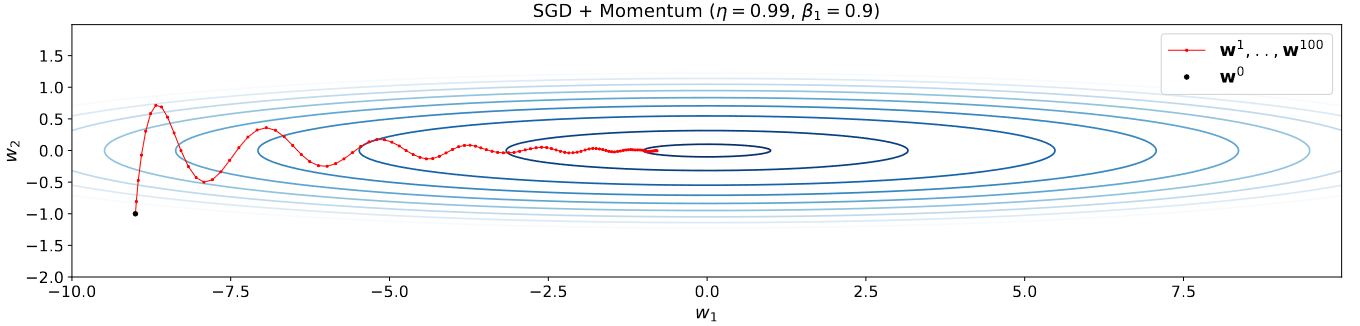
\includegraphics[width=1\textwidth]{assets/pics/sgd-momentum.png}
    \captionsource{Ilustrasi dari pembaruan parameter $\bm{\theta}=\{w_1, w_2\}$ dengan \f{stochastic gradient descent} dengan momentum.}{\citep{geiger2022deeplearning}.}
    \label{fig:sgd-momentum}
\end{figure}

Metode lainnya yang dapat digunakan untuk mempercepat proses pembaruan parameter $\bm{\theta}$ adalah metode \f{adaptive learning rate}. Metode \f{adaptive learning rate} mengubah \f{learning rate} pada setiap parameter $\bm{\theta}$ dengan membagi \f{learning rate} awal dengan \f{moving average} dari kuadrat gradien -- biasanya disebut sebagai \f{running variance} -- pada parameter $\bm{\theta}$ tersebut. Pembagian antara gradien dan \f{running variance} tersebut dilakukan secara \f{element-wise}. \equ~\ref{eq:rmsprop} menunjukkan algoritma \f{stochastic gradient descent} dengan \f{adaptive learning rate} dan \pic~\ref{fig:rmsprop} menngilustrasikan pembaruan parameter $\bm{\theta}$ dengan \f{adaptive learning rate}.
\begin{align}
    \label{eq:rmsprop}
    \bm{\theta}^{(t+1)} &= \bm{\theta}^{(t)} - \frac{\eta \nabla_{\bm{\theta}} L_{\mathcal{B}}(\bm{\theta}^{(t)})}{\sqrt{\mathbf{v}^{(t+1)}} + \epsilon}, \\
    \mathbf{v}^{(t+1)} &= \beta_2 \mathbf{v}^{(t)} + (1 - \beta_2) \left(\nabla_{\bm{\theta}} L_{\mathcal{B}}(\bm{\theta}^{(t)})\odot \nabla_{\bm{\theta}} L_{\mathcal{B}}(\bm{\theta}^{(t)})\right),
\end{align}
dengan $\beta_2 \in [0, 1)$ dan $\odot$ adalah operasi perkalian \f{element-wise} antara dua matriks atau vektor.
\begin{figure}[!ht]
    \centering
    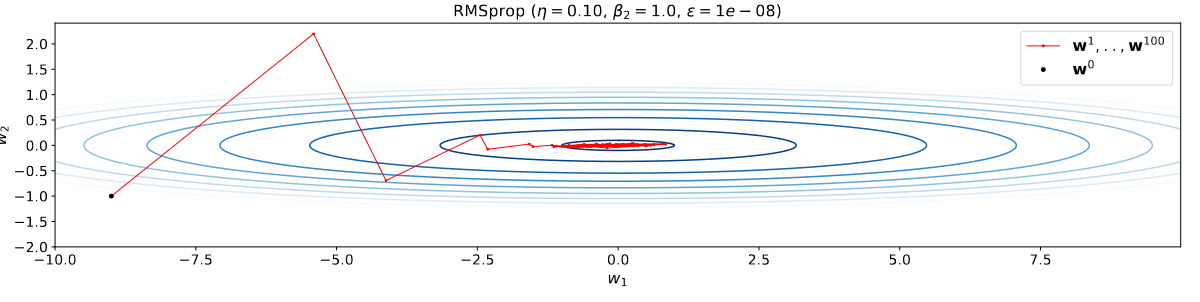
\includegraphics[width=1\textwidth]{assets/pics/RMSPROP.png}
    \captionsource{Ilustrasi dari pembaruan parameter $\bm{\theta}=\{w_1, w_2\}$ dengan \f{adaptive learning rate}.}{\citep{geiger2022deeplearning}.}
    \label{fig:rmsprop}
\end{figure}

Faktor $\epsilon$ yang ditambahkan pada \equ~\ref{eq:rmsprop} digunakan untuk menghindari pembagian dengan nol pada awal iterasi karena inisialiasi awal vektor $\mathbf{v}^{(0)}$ adalah nol.

Terakhir, metode optimasi \f{Adaptive Moment Estimation} (Adam) menggabungkan metode \f{stochastic gradient descent} dengan momentum dan \f{adaptive learning rate}. \equ~\ref{eq:adam} menunjukkan algoritma \f{stochastic gradient descent} dengan Adam dan \pic~\ref{fig:adam} mengilustrasikan pembaruan parameter $\bm{\theta}$ dengan Adam. \equ~\ref{eq:adam} menunjukkan persamaan dari metode optimasi Adam dan \pic~\ref{fig:adam} mengilustrasikan pembaruan parameter $\bm{\theta}$ dengan Adam.
\begin{figure}[!ht]
    \centering
    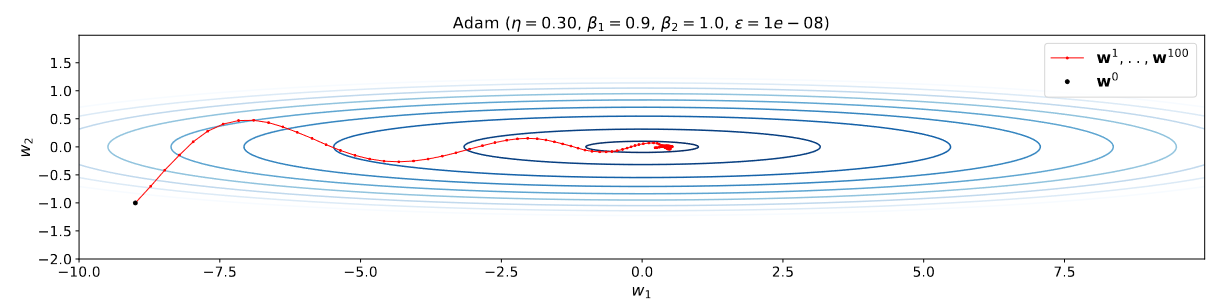
\includegraphics[width=1\textwidth]{assets/pics/adam.png}
    \captionsource{Ilustrasi dari pembaruan parameter $\bm{\theta} = \{w_1, w_2\}$ dengan Adam.}{\citep{geiger2022deeplearning}.}
    \label{fig:adam}
\end{figure}
\begin{align}
    \label{eq:adam}
    \bm{\theta}^{(t+1)} &= \bm{\theta}^{(t)} - \frac{\eta \hat{\mathbf{m}}^{(t+1)}}{\sqrt{\hat{\mathbf{v}}^{(t+1)}} + \epsilon}, \\
    \label{eq:adam-momemntum-with-bias-correction}
    \hat{\mathbf{m}}^{(t+1)} &= \frac{\mathbf{m}^{(t+1)}}{1 - \beta_1}, \\
    \label{eq:adam-running-variance-with-bias-correction}
    \hat{\mathbf{v}}^{(t+1)} &= \frac{\mathbf{v}^{(t+1)}}{1 - \beta_2}, \\
    \mathbf{m}^{(t+1)} &= \beta_1 \mathbf{m}^{(t)} + (1 - \beta_1) \nabla_{\bm{\theta}} L_{\mathcal{B}}(\bm{\theta}^{(t)}), \\
    \mathbf{v}^{(t+1)} &= \beta_2 \mathbf{v}^{(t)} + (1 - \beta_2) \left(\nabla_{\bm{\theta}} L_{\mathcal{B}}(\bm{\theta}^{(t)})\odot \nabla_{\bm{\theta}} L_{\mathcal{B}}(\bm{\theta}^{(t)})\right).
\end{align}

Alasan dilakukan pembagian dengan $(1-\beta_1)$ dan $(1-\beta_2)$ \equ~\ref{eq:adam-momemntum-with-bias-correction} dan \equ~\ref{eq:adam-running-variance-with-bias-correction} adalah untuk menghilangkan bias pada \f{momentum} dan \f{running variance} pada awal iterasi.


\section{Pembelajaran Representasi}
Pembelajaran representasi adalah proses pembelajaran model \f{machine learning} atau \f{deep learning} $f_{\text{model}}(x): \mathcal{X} \rightarrow \mathbb{R}^n$ yang memetakan \f{high dimensional input} $x \in \mathcal{X}$ ke dalam ruang vektor $\mathbb{R}^n$. Pemetaan yang diharapkan dari model $f_{\text{model}}(x)$ diharapkan dapat mengenkode informasi yang terkandung pada $x$ ke dalam vektor $\mathbf{R}^n$. Salah satu contoh informasi yang dapat dienkode adalah jarak antara dua kalimat $x_1$ dan $x_2$ yang memiliki kesamaan semantik atau sintaksis akan lebih dekat daripada jarak antara dua kalimat $x_1$ dan $x_3$ yang tidak memiliki kesamaan sama sekali pada ruang vektor. \pic~\ref{fig:reps-learning} mengilustrasikan pemetaan \f{input} menjadi vektor.
\begin{figure}[!ht]
    \centering
    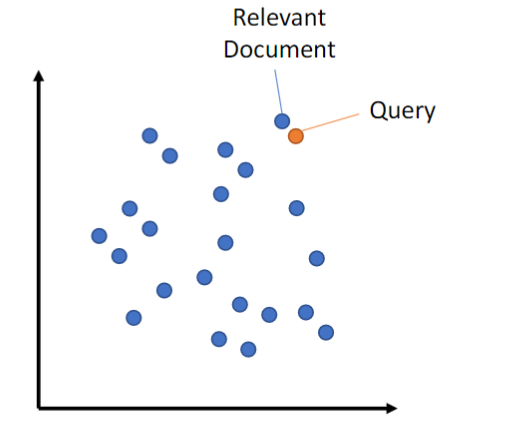
\includegraphics[width=0.5\textwidth]{assets/pics/reps-learning.png}
    \captionsource{Ilustrasi dari Pemetaan \f{input} menjadi vektor. \f{input} yang memiliki kesamaan semantik atau sintaksis akan lebih dekat daripada \f{input} yang tidak memiliki kesamaan.}{\url{https://www.sbert.net}}
    \label{fig:reps-learning}
\end{figure}

\subsection{Fungsi \f{Loss} pada Pembelajaran Representasi}


Fungsi loss pada pembelajaran representasi untuk permasalahan pemeringkatan teks biasanya disebut sebagai \f{ranking loss}. Meminimalkan fungsi \f{ranking loss} berarti memastikan bahwa \f{input-input} yang serupa berada lebih dekat daripada \f{input-input} yang tidak mirip. Sebagian besar fungsi loss pada pembelajaran representasi tidak memerlukan label kelas.

Fungsi loss yang digunakan pada penelitian ini adalah \f{N-pair loss} \citep{InfoNCE}. \f{N-pair loss} dapat ditinjau sebagai klasifikasi multikelas dengan N-1 kelas berupa kelas negatif (kelas yang tidak mirip dengan \f{input} yang diberikan) dan 1 kelas positif (kelas yang mirip dengan \f{input} yang diberikan). Untuk suatu \f{input} $x$ dan \f{input} positif $x^+$ dan kumpulan \f{input} negatif $\{x^-_i\}_{i=1}^{N-1}$, \f{N-pair loss} dapat ditulis seperti pada \equ~\ref{eq:n-pair-loss}.
\begin{align}
\label{eq:n-pair-loss}
\nonumber
 L(x, x^+, \{x^-_i\}_{i=1}^{N-1}) = \\
 -\log\frac{\exp(\text{sim}((f_\text{model}(x), f_\text{model}(x^+)))}{\sum_{i=1}^{N-1} \exp(\text{sim}(f_\text{model}(x), f_\text{model}(x^-_i)))+\exp(\text{sim}(f_\text{model}(x), f_\text{model}(x^+)))},
\end{align}
dengan $\text{sim}$ adalah fungsi yang mengukur keserupaan antara dua vektor (fungsi jarak). Pada penelitian ini, fungsi $\text{sim}$ yang digunakan adalah fungsi \f{dot product} sehingga \equ~\ref{eq:n-pair-loss} dapat ditulis ulang seperti pada \equ~\ref{eq:n-pair-loss-dot-product}.
\begin{align}
\label{eq:n-pair-loss-dot-product}
 L(x, x^+, \{x^-_i\}_{i=1}^{N-1}) &= -\log\frac{\exp(f_\text{model}(x)^{\top}f_\text{model}(x^+))}{\sum_{i=1}^{N-1} \exp(f_\text{model}(x)^{\top}f_\text{model}(x^-_i))+\exp(f_\text{model}(x)^{\top}f_\text{model}(x^+))}.
\end{align}

\pic~\ref{fig:n-pair-loss} mengilustrasikan fungsi \f{N-pair loss}. Untuk pasangan teks yang relevan $(a, b_1)$, tujuannya adalah untuk meminimalkan jarak (fungsi sim) antara $a$ dan $b_1$ sehingga jarak tersebut lebih kecil dibandingkan dengan jarak antara $a$ dan $b_i$ yang lain.
\begin{figure}[!ht]
    \centering
    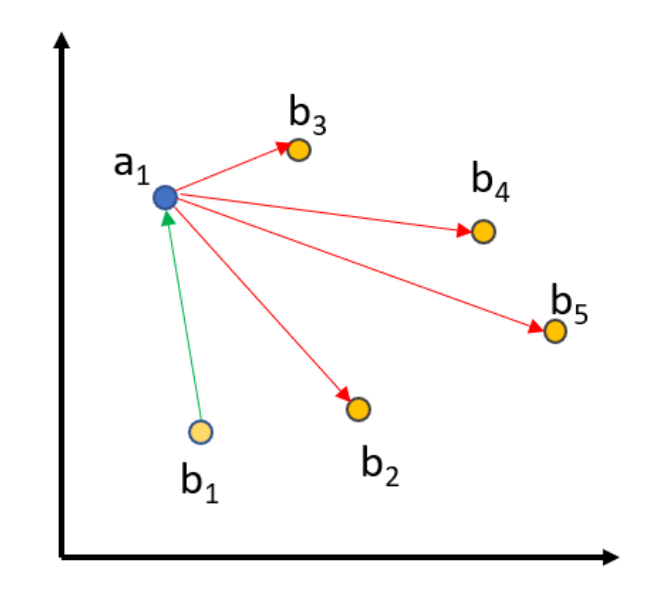
\includegraphics[width=0.5\textwidth]{assets/pics/InfoNCE.png}
    \captionsource{Ilustrasi fungsi objektif \f{N-pair loss}. Untuk pasangan teks yang relevan $(a, b_1)$, tujuannya adalah untuk meminimalkan jarak antara $a$ dan $b_1$ sehingga jarak tersebut lebih kecil dibandingkan dengan jarak antara $a$ dan $b_i$ yang lain.}{\url{https://www.sbert.net/}}
    \label{fig:n-pair-loss}
\end{figure}

















        

